\chapter{The Superstition of Waves}

\section{The Addition of Waves}

\subsection{The Algebraic Method}

\begin{equation*}
  \begin{aligned}
    E \left( x, t \right) = E_0 \sin \left[ \omega t - \left( k x + \varepsilon \right) \right]
  \end{aligned}
\end{equation*}

let

\begin{equation*}
  \begin{aligned}
    \alpha \left( x , \varepsilon \right) = - \left( k x + \varepsilon \right)
  \end{aligned}
\end{equation*}

Then

\begin{equation*}
  \begin{aligned}
    E \left( x , t \right) = E_0 \sin \left[ \omega t + \alpha \left( x , \varepsilon \right) \right]
  \end{aligned}
\end{equation*}

Two waves of the same frequency

\begin{equation*}
  \left\{
    \begin{aligned}
      & E_1 = E_{01} \sin \left( \omega t + \alpha_1 \right) \\
      & E_2 = E_{02} \sin \left( \omega t + \alpha_2 \right) 
    \end{aligned}
  \right.
\end{equation*}

\begin{equation*}
  \begin{aligned}
    E = E_1 + E_2 &= E_{01} \left( \sin \omega t \cos \alpha_1 + \cos \omega t \sin \alpha_1 \right) + E_{02} \left( \sin \omega t \cos \alpha_2 + \cos \omega t \sin \alpha_2  \right) \\
    &= \left( E_{01} \cos \alpha_1 + E_{02} \cos \alpha_2 \right) \sin \omega t + \left( E_{01} \sin \alpha_1 + E_{02} \sin \alpha_2 \right) \cos \omega t \\
    &= E_0 \cos \alpha \sin \omega t + E_0 \sin \alpha \cos \omega t \\
    &= E_0 \sin \left( \omega t + \alpha \right)
  \end{aligned}
\end{equation*}

\begin{equation*}
  \left\{
    \begin{aligned}
      & E_0 \cos \alpha = E_{01} \cos \alpha_1 + E_{02} \cos \alpha_2 \\
      & E_0 \sin \alpha = E_{01} \sin \alpha_1 + E_{02} \sin \alpha_2 \\
    \end{aligned}
  \right.
  \Rightarrow
  \left\{
    \begin{aligned}
      & E_0^2 = E_{01}^2 + E_{02}^2 + 2 E_{01} E_{02} \cos \left( \alpha_2 - \alpha_1 \right) \\
      & \tan \alpha = \dfrac{E_{01} \sin \alpha_1 + E_{02} \sin \alpha_2}{E_{01} \cos \alpha_1 + E_{02} \cos \alpha_2} 
    \end{aligned}
  \right.
\end{equation*}

The phase difference

\begin{equation*}
  \begin{aligned}
    \delta = \left( k x_1 + \varepsilon_1 \right) - \left( k x_2 + \varepsilon_2 \right) = \dfrac{2 \pi}{\lambda} \left( x_1 - x_2 \right) + \left( \varepsilon_1 - \varepsilon_2 \right)
  \end{aligned}
\end{equation*}

When $E_{01} = E_{02}$ and $\alpha_2 - \alpha_1 = \Delta x$
\begin{equation*}
  \begin{aligned}
      & E_0^2 = 2 E_{01}^2 + 2 E_{01}^2 \cos \left( k \Delta x \right) = 2 E_{01}^2 \left[ 1 + \cos \left( k \Delta x \right) \right] \\
  \end{aligned}
\end{equation*}

\begin{equation*}
  \begin{aligned}
    \cos 2x = 2 \cos^2 x - 1 \Rightarrow \cos \left( k \Delta x \right) = 2 \cos^2 \left( \dfrac{k \Delta x}{2}  \right) - 1
  \end{aligned}
\end{equation*}

$\Rightarrow$

\begin{equation*}
  \begin{aligned}
    E_0^2 = 2 E_{01}^2 \cos^2 \left( \dfrac{k \Delta x}{2}  \right)
  \end{aligned}
\end{equation*}

Period of the amplitude of addition

\begin{equation*}
  \begin{aligned}
    \dfrac{k \Delta x}{2} = \dfrac{\pi}{2}  \Rightarrow k \left( \alpha_2 - \alpha_1 \right) = \pi \Rightarrow \Delta x = \alpha_2 - \alpha_1 = \dfrac{\lambda}{2} 
  \end{aligned}
\end{equation*}

\subsection{The Complex Method}

\begin{equation*}
  \begin{aligned}
    E_1 = E_{01} \cos \left( kx \pm \omega t \right) \Rightarrow \tilde{E}_1 = E_{01} \exp \left[ i \left( k x \pm \omega t \right) \right]
  \end{aligned}
\end{equation*}

\begin{equation*}
  \left\{
    \begin{aligned}
      & E_1 = E_{01} \exp \left[ i \alpha_1 \right] \\
      & E_2 = E_{02} \exp \left[ i \alpha_2 \right] \\
      & E_0 = E_1 + E_2
    \end{aligned}
  \right.
\end{equation*}

\begin{equation*}
  \begin{aligned}
    E_0^2 &= \left( E_{01} \exp \left[ i \alpha_1 \right] + E_{02} \exp \left[ i \alpha_2 \right] \right) \cdot \left( E_{01} \exp \left[ - i \alpha_1 \right] + E_{02} \exp \left[ - i \alpha_2 \right] \right) \\
    &= E_{01}^2 + E_{02}^2 + 2 E_{01} E_{02} \cos \left( \alpha_1 - \alpha_2 \right)
  \end{aligned}
\end{equation*}

\subsection{Phasor Addition Method}

\begin{figure}[H]
  \centering
  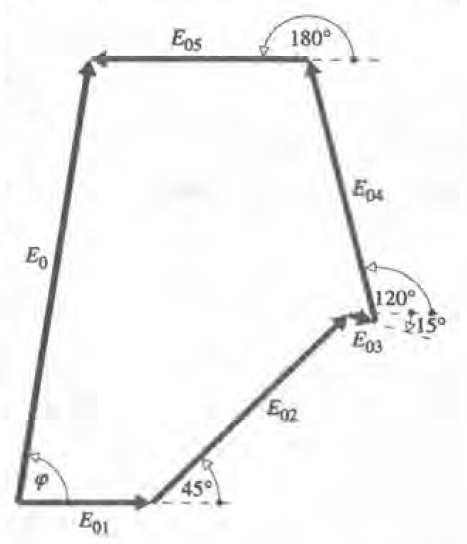
\includegraphics[width=0.3\linewidth]{figures/Phasor-Addition}
  \caption{Phasor Addition Method}
  \label{fig:}
\end{figure}

\section{Standing Waves}

\begin{equation*}
  \begin{aligned}
    & E_L = E_{0t} \sin \left( k x - \omega t \right) \\
    & E_R = E_{0t} \sin \left( k x - \omega t \right)
    & E = E_L + E_R
  \end{aligned}
\end{equation*}

\begin{equation*}
  \begin{aligned}
    \sin \alpha + \sin \beta = 2 \sin \dfrac{\alpha + \beta}{2} \cos \dfrac{\alpha - \beta}{2}  
  \end{aligned}
\end{equation*}

$\Rightarrow$

\begin{equation*}
  \begin{aligned}
    E = 2 E_{0t} \sin kx \cos \omega t
  \end{aligned}
\end{equation*}

\section{Addition of Waves of Different Frequency}

\begin{equation*}
  \left\{
    \begin{aligned}
      & E_1 = E_{01} \cos \left( k_1 x - \omega_1 t \right) \\
      & E_2 = E_{02} \cos \left( k_2 x - \omega_2 t \right) \\
      & E = E_1 + E_2
    \end{aligned}
  \right.
\end{equation*}

\begin{equation*}
  \begin{aligned}
    \cos \alpha + \cos \beta = 2 \cos \dfrac{\alpha + \beta}{2} \cos \dfrac{\alpha - \beta}{2}  
  \end{aligned}
\end{equation*}



$\Rightarrow$

\begin{equation*}
  \begin{aligned}
    E &= E_{01} \left[ \cos \left( k_1 x - \omega t \right) + \cos \left( k_2 x - \omega_2 t \right) \right] \\
    &= 2 E_{01} \cos \dfrac{1}{2} \left[ \left( k_1 + k_2 \right) x - \left( \omega_1 + \omega_2 \right) t \right] \times \cos \dfrac{1}{2} \left[ \left( k_1 - k_2 \right) x - \left( \omega_1 - \omega_2 \right) t \right]  
  \end{aligned}
\end{equation*}

Define

\begin{equation*}
  \begin{aligned}
    & \bar{\omega} = \dfrac{1}{2} \left( \omega_1 + \omega_2 \right) \\ 
    & \bar{k} = \dfrac{1}{2} \left( k_1 + k_2 \right) \\
  \end{aligned}
  \quad\quad\quad\quad
  \begin{aligned}
      & \omega_m = \dfrac{1}{2} \left( \omega_1 - \omega_2 \right) \\ 
      & k_m = \dfrac{1}{2} \left( k_1 - k_2 \right) 
  \end{aligned}
\end{equation*}

Then

\begin{equation*}
  \begin{aligned}
    E = 2 E_{01} \cos \left( k_m x - \omega_m t \right) \cos \left( \bar{k} x - \bar{\omega} t \right) = E_0 \left( x , t \right) \cos \left( \bar{k} x - \bar{\omega} t \right)
  \end{aligned}
\end{equation*}

Noted that

\begin{equation*}
  \begin{aligned}
    & \bar{\omega} = \dfrac{1}{2} \left( \omega_1 + \omega_2 \right) \\ 
    & \bar{k} = \dfrac{1}{2} \left( k_1 + k_2 \right) \\
  \end{aligned}
  \quad\quad \gg \quad\quad
  \begin{aligned}
      & \omega_m = \dfrac{1}{2} \left( \omega_1 - \omega_2 \right) \\ 
      & k_m = \dfrac{1}{2} \left( k_1 - k_2 \right) 
  \end{aligned}
\end{equation*}

$E_0 = 2 E_{01} \cos \left( k_m x - \omega_m t \right)$ varies far less frequently than $\cos \left( \bar{k} x - \bar{\omega} t \right)$

\begin{figure}[H]
  \centering
  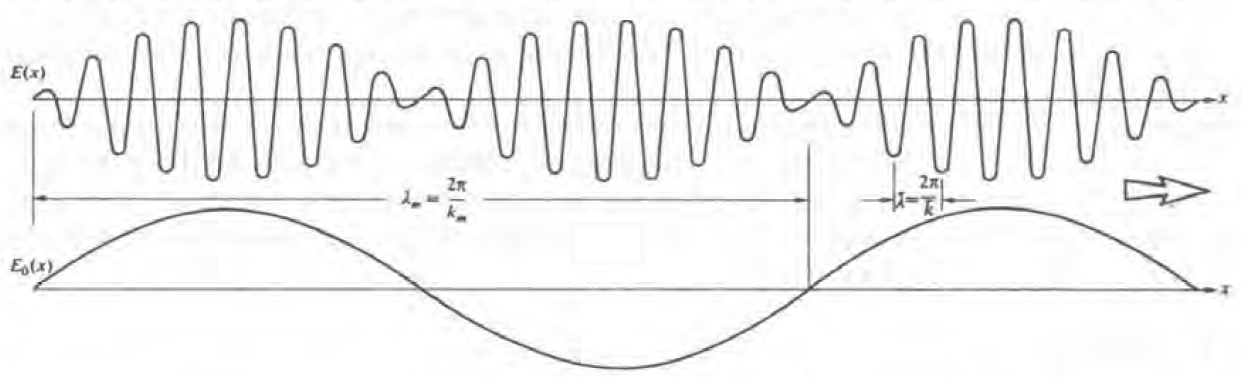
\includegraphics[width=\linewidth]{figures/Standing-Wave}
  \caption{Standing Wave}
  \label{fig:}
\end{figure}

\begin{table*}[h]
  \centering
  \begin{tabular}{|Sc|Sc|}
    \hline
    Beat Frequency (Time) & $2 \omega_m $ \\
    \hline
    Beat Frequency (Space) & $ 2 k_m $ \\
    \hline
  \end{tabular}
  \quad\quad\quad\quad
  \begin{tabular}{|Sc|Sc|}
    \hline
    Group Frequency & $v_g = \omega_m / k_m $ \\
    \hline
    Phase Velocity & $ v_p = \bar{\omega} / \bar{k}$ \\
    \hline
  \end{tabular}
\end{table*}

\section{Light in Dispersible Media}

\begin{table*}[h]
  \centering
  \begin{tabular}{|Sc|Sc|}
    \hline
    Average Phase Velocity & $\bar{v}_p = \dfrac{c}{\bar{n}} $ \\
    \hline
    Group Velocity & $v_g = \dfrac{c}{\bar{n}} \left( 1 + \dfrac{\bar{\lambda}}{\bar{n}} \dfrac{\Delta n}{\Delta \lambda}   \right) $ \\
    \hline
  \end{tabular}
  \quad\quad\quad\quad
  \begin{tabular}{|Sc|Sc|}
    \hline
    Normal Dispersion Media & $\bar{v}_p > v_g $ \\
    \hline
    Anomalous Dispersion Media & $ \bar{v}_p < v_g $ \\
    \hline
  \end{tabular}
\end{table*}


%%% Local Variables:
%%% mode: latex
%%% TeX-master: "Optics"
%%% End:
